\documentclass[11pt]{article}
\usepackage[letterpaper,margin=1in]{geometry}
\usepackage[T1]{fontenc}
\usepackage{lmodern}
\usepackage{amsmath,amssymb,amsthm,booktabs,microtype,xcolor,tikz,needspace}
\usetikzlibrary{arrows.meta}
\usepackage[colorlinks=true,linkcolor=blue!45!black,urlcolor=blue!45!black,citecolor=blue!45!black]{hyperref}
\newtheorem{theorem}{Theorem}[section]
\newtheorem{lemma}[theorem]{Lemma}
\newtheorem{proposition}[theorem]{Proposition}
\newtheorem{corollary}[theorem]{Corollary}
\newcommand{\cind}{c_{\mathrm{ind}}}
\setlength{\emergencystretch}{2em}
\raggedbottom
\hypersetup{pdftitle={Two induced cycle subgraphs in cubic graphs with a square factor},
pdfsubject={Partial progress on the induced cycles conjecture; the general conjecture is not solved}}
\title{Two Induced Cycle Subgraphs in Cubic Graphs\\with a Square Factor}
\author{}
\date{October 26, 2026}
\begin{document}
\maketitle
\begin{abstract}
The induced cycles conjecture of Henning, Joos, L\"owenstein and Sasse
asks whether every cubic graph of order $n$ contains an induced
$2$-regular subgraph of order at least $n/2$.
We prove the assertion for every cubic graph admitting a square factor.
More strongly, two induced $2$-regular subgraphs can be constructed whose
vertex sets cover the graph, have equal cardinality, and intersect in an
induced matching. Consequently an induced $2$-regular subgraph captures
at least half of any prescribed nonnegative vertex weight.
The proof alternately colors an Euler circuit after contracting the
squares, then repairs opposite pairs by orienting the resulting
$2$-factors. We give an exact formula for a family of square necklaces
and an explicit ten-vertex obstruction to extending the two-subgraph
cover assertion to all bridgeless cubic graphs.
A standard-library verifier accompanies the proofs.
These results are partial progress: the general cubic conjecture
is neither proved nor disproved here.
\end{abstract}
\noindent\textbf{Keywords.} Cubic graph; induced regular subgraph;
square factor; Euler circuit; vertex weights.

\section{The open problem and the scope of this note}
All graphs under consideration are finite. The input graph $G$ is simple
and cubic, meaning that every vertex has degree three.
A set $S\subseteq V(G)$ is \emph{good} if $G[S]$ is $2$-regular.
Thus its components are cycles, and all edges of $G$ between vertices
of $S$ belong to those cycles. The empty set is allowed. Write
\[
 \cind(G)=\max\{|S|: S\text{ is good}\}.
\]
Henning, Joos, L\"owenstein and Sasse proposed the following in their
2014 preprint, subsequently published in 2016 \cite{HJLS}:
\begin{equation}\label{eq:conjecture}
 \cind(G)\geq \frac{|V(G)|}{2}\qquad\text{for every cubic graph }G.
\end{equation}
Their general lower bound is $(n+2)/4$, and their claw-free bound is
strictly greater than $13n/20$.
August and October 2026 papers still treat \eqref{eq:conjecture} as
unresolved \cite{KSS,RRT}. The literature check for this note was
performed on October 26, 2026.

A \emph{square factor} is a spanning $2$-regular subgraph all of whose
components have order four. Its squares need not be induced in $G$:
a chord is permitted. This condition is different from being
$4$-chordal, which forbids all induced cycles longer than four.
The result below is proved directly and includes no computational step.
Targeted searches did not locate this specific square-factor
statement; that search does not establish publication priority.
No claim to solve \eqref{eq:conjecture} in general is made.

\begin{theorem}[Two induced cycle subgraphs]\label{thm:main}
Let $G$ be a cubic graph with a specified square factor on $q$ squares,
so that $n=4q$. There are good sets $A,B\subseteq V(G)$ and an integer
$b\geq0$ such that
\[
 A\cup B=V(G),\qquad |A|=|B|=2q+b,\qquad |A\cap B|=2b.
\]
The graph induced by $A\cap B$ is a matching of $b$ edges.
In particular, $\cind(G)\geq n/2$.
Given the factor, the construction can be implemented in $O(n)$ time.
\end{theorem}

The constant $1/2$ cannot be increased for this class: the twelve-vertex
square necklace in Section~\ref{sec:necklace} has $\cind=6$.

\begin{corollary}[Nonnegative vertex weights]\label{cor:weighted}
Under the assumptions of Theorem~\ref{thm:main}, let
$w:V(G)\to[0,\infty)$ and $w(X)=\sum_{v\in X}w(v)$.
One can construct a good set $S$ satisfying
\[
 w(S)\geq \tfrac12 w(V(G)).
\]
\end{corollary}
\begin{proof}
For the two sets in the theorem,
$w(A)+w(B)=w(V(G))+w(A\cap B)\geq w(V(G))$.
Choose the set of larger weight.
\end{proof}

\section{Contraction and the local repair}
Let $F$ be the square factor and let $M=E(G)\setminus E(F)$.
Since $G$ is cubic, $M$ is a perfect matching.
Contract each square of $F$ to a single vertex while retaining all edges
of $M$. The resulting multigraph $Q$ is $4$-regular, with loops counted
twice in the degree. Each incidence at a vertex of $Q$ corresponds to
one of the four original vertices of its square; call that vertex
the \emph{port} of the incidence. A chord of a square becomes a loop
with two different ports.

\begin{lemma}\label{lem:factor}
The edges of a finite $4$-regular multigraph can be partitioned into
two $2$-factors $R$ and $B$.
\end{lemma}
\begin{proof}
Take an Euler circuit in each connected component and color its edges
alternately red and blue. A component on $r$ vertices has $2r$ edges,
so the alternation is consistent at the closing point. At every
vertex, each arrival is paired with the following departure, and
each such pair has one incidence of each color. Thus every vertex has
two red and two blue incidences. This argument includes loops.
\end{proof}

Call a square \emph{split} if its two red ports are opposite on its
four-cycle. This occurs if and only if its two blue ports are opposite.
Otherwise the red ports are adjacent, and the blue ports are adjacent.
Let $b$ be the number of split squares.

Orient every component of $R$ cyclically and do the same for $B$.
A component may be a loop or two parallel edges; in every case each
vertex has one incoming and one outgoing incidence of each color.
For a color $c$, write $T_c$ for the set of all ports of color $c$.
Define
\begin{equation}\label{eq:construction}
 S_c=T_c\ \cup\
 \{\text{outgoing port of the other color in each split square}\}.
\end{equation}
For a loop, the outgoing port means exactly one of its two distinct
original endpoints, as determined by its orientation.

\begin{figure}[ht]
\centering
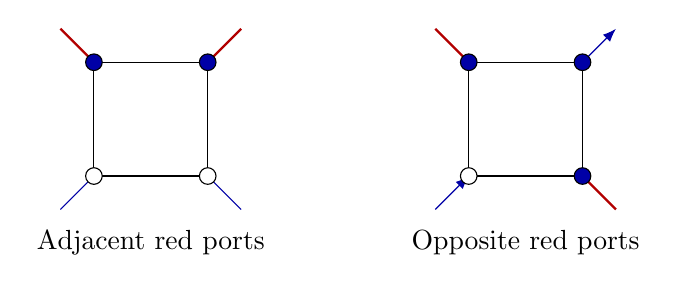
\begin{tikzpicture}[scale=0.85,
selected/.style={circle,draw,fill=blue!65!black,minimum size=6pt,inner sep=0pt},
unselected/.style={circle,draw,fill=white,minimum size=6pt,inner sep=0pt}]
\begin{scope}
 \draw (0,0)--(1.7,0)--(1.7,1.7)--(0,1.7)--cycle;
 \draw[thick,red!70!black] (0,1.7)--(-.5,2.2) (1.7,1.7)--(2.2,2.2);
 \draw[blue!65!black] (0,0)--(-.5,-.5) (1.7,0)--(2.2,-.5);
 \node[selected] at (0,1.7){};
 \node[selected] at (1.7,1.7){};
 \node[unselected] at (0,0){};
 \node[unselected] at (1.7,0){};
 \node at (.85,-1) {Adjacent red ports};
\end{scope}
\begin{scope}[xshift=5.6cm]
 \draw (0,0)--(1.7,0)--(1.7,1.7)--(0,1.7)--cycle;
 \draw[thick,red!70!black] (0,1.7)--(-.5,2.2) (1.7,0)--(2.2,-.5);
 \draw[blue!65!black,-{Latex}] (1.7,1.7)--(2.2,2.2);
 \draw[blue!65!black,-{Latex}] (-.5,-.5)--(0,0);
 \node[selected] at (0,1.7){};
 \node[selected] at (1.7,0){};
 \node[selected] at (1.7,1.7){};
 \node[unselected] at (0,0){};
 \node at (.85,-1) {Opposite red ports};
\end{scope}
\end{tikzpicture}
\caption{Construction of $S_{\rm red}$. Filled vertices are selected.
In a split square, the outgoing blue port is added, forming a
three-vertex path. The orientation prevents both ends of a blue
matching edge from being added.}
\label{fig:repair}
\end{figure}

\Needspace{7\baselineskip}
\begin{lemma}\label{lem:good}
Each set $S_c$ defined in \eqref{eq:construction} is good.
\end{lemma}
\begin{proof}
Consider $c={\rm red}$; the other case is identical.
In a nonsplit square, the two selected red ports are adjacent.
Each has one selected neighbor within the four-cycle. Its matching
edge is red, so its matching partner is also selected. Its other
four-cycle neighbor is unselected. Its degree in $G[S_{\rm red}]$
is therefore exactly two.

In a split square, the two red ports and the chosen blue port form a
three-vertex path. Each red port has one selected four-cycle neighbor
and its selected red matching partner, hence degree two.
The added blue port has its two red four-cycle neighbors selected.
Its blue matching partner is unselected: at the head of an oriented
blue edge the incoming blue port is never added. The partner is not
a red port either. This remains true for a loop, whose incoming and
outgoing ports are different original vertices.
Thus the added blue port also has degree exactly two.
These are all selected vertices.
\end{proof}

\begin{proof}[Proof of Theorem~\ref{thm:main}]
Set $A=S_{\rm red}$ and $B=S_{\rm blue}$.
Every original vertex is a port of exactly one color, so $T_{\rm red}$
and $T_{\rm blue}$ partition $V(G)$ and consequently $A\cup B=V(G)$.
Each set includes two ports per square and one extra port in each
split square. This proves $|A|=|B|=2q+b$.

A nonsplit square contributes no vertex to $A\cap B$.
A split square contributes its outgoing red and outgoing blue ports.
They are adjacent, since red and blue ports alternate around that
square. No matching edge joins two intersection vertices: an
intersection port is outgoing in the orientation of its color, whereas
the other endpoint of that matching edge is incoming.
There are no other edges between different squares.
Thus the intersection induces precisely one edge per split square.

For the running time, build $Q$, find Euler circuits by
Hierholzer's algorithm, alternate the colors, traverse the monochromatic
circuits to orient them, and apply \eqref{eq:construction}.
Each step takes linear time in the size of $Q$ or $G$.
The factor is part of the input; this is not a claim about the time
needed to find a square factor in an arbitrary cubic graph.
\end{proof}

\section{An exact family and sharpness}\label{sec:necklace}
For $k\geq2$, define $N_k$ using blocks
\[
 L_i=\{\ell_i^0,\ell_i^1\},\qquad
 R_i=\{r_i^0,r_i^1\}\qquad (i\in\mathbb Z/k\mathbb Z).
\]
Within block $i$, include all four edges between $L_i$ and $R_i$.
Also include the matching edges $r_i^j\ell_{i+1}^j$ for $j=0,1$.
This is a simple cubic graph on $4k$ vertices with the specified square
factor.

\Needspace{8\baselineskip}
\begin{theorem}\label{thm:necklace}
For every $k\geq2$,
\[
 \cind(N_k)=
 \begin{cases}
  3k,& k\text{ even},\\
  3k-3,& k\text{ odd}.
 \end{cases}
\]
In particular, $\cind(N_3)=6=|V(N_3)|/2$.
\end{theorem}
\begin{proof}
Let $S$ be good and record the number of selected vertices in each
block. The possible block sizes are $0,2,3,4$.
Size one is impossible, since a lone selected vertex has at most its
matching neighbor. In size two, the vertices must lie in opposite
parts $L_i,R_i$, hence be adjacent.

The following local restrictions will suffice.
\begin{enumerate}
\item A size-four block forces both neighboring blocks to have size
zero. All four matching partners of its vertices must be unselected.
At either neighboring block this excludes one entire part, and a
nonempty subset of the other part cannot have selected degree two.
For $k=2$, both parts of the same neighboring block are excluded.
\item A size-three block selects both vertices of one part and one of
the other. The selected pair requires both matching partners in the
neighboring block on that side. That neighbor is consequently also
a size-three block, with its selected pair facing back.
It cannot have size four by the first restriction.
Thus size-three blocks occur in mutually facing pairs.
\item Size-two and size-three blocks cannot be neighbors.
If the pair in the size-three block faces the size-two block, the
latter would have to select both vertices of a part.
If the singleton faces it, that singleton requires its matching
partner to be unselected, and the other port on that side is itself
unselected. Neither port on the size-two side can then have a selected
matching partner, which its selected vertex requires.
\end{enumerate}

Let $z,t,p,f$ count the blocks of sizes $0,2,3,4$, respectively.
The selected order is
\begin{equation}\label{eq:count}
 |S|=2t+3p+4f=3k-3z-t+f.
\end{equation}
Every size-four block can be mapped to its next block, which has size
zero; this map is injective, so $z\geq f$.
Equation~\eqref{eq:count} therefore gives $|S|\leq3k$.

Suppose now that $k$ is odd, hence $k\geq3$.
If $f=1$, the size-four block has two distinct zero neighbors, giving
$3z+t-f\geq5$. If $f\geq2$, then $3z+t-f\geq2f\geq4$.
If $f=0$ and $z\geq1$, this deficit is at least three.
It remains to consider $f=z=0$.
By the third restriction and the connectivity of the cyclic sequence,
all blocks then have size two or all have size three.
The latter is impossible for odd $k$ by the pairing restriction.
In the former case $|S|=2k\leq3k-3$.
Thus $|S|\leq3k-3$ for odd $k$.

For attainment when $k$ is even, pair consecutive blocks.
In the first block of each pair select both right vertices and one
left vertex; in the second select both left vertices and one right
vertex. At the boundary between successive pairs choose the two
singletons with different superscripts. Their matching partners are
then unselected. All selected vertices have degree two, giving $3k$
vertices.

When $k$ is odd, leave one block empty and pair the remaining $k-1$
blocks consecutively. Use the same choice between pairs. The two
outer singletons have their matching partners in the empty block.
This gives $3(k-1)$ selected vertices.
\end{proof}
The example $N_3$ supplies an exact obstruction to improving the
unweighted constant, and uniform vertex weights give the same
sharpness for Corollary~\ref{cor:weighted}.

\section{Why the two-subgraph method does not settle the conjecture}
The covering assertion of Theorem~\ref{thm:main} is stronger than
\eqref{eq:conjecture}. It already fails for a small connected bridgeless
cubic graph.

\begin{proposition}\label{prop:obstruction}
There is a connected bridgeless cubic graph $H$ on ten vertices such
that $\cind(H)=6$, but no two good sets have union $V(H)$.
\end{proposition}
\begin{proof}
Take two disjoint diamonds $D_i$ with vertices $a_i,b_i,c_i,d_i$,
where the missing edge is $a_ib_i$. Add two vertices $x,y$, the edge
$xy$, and the four edges $xa_i,yb_i$ for $i=1,2$.
All degrees are three. The diamond edges lie on triangles; each
attachment edge and $xy$ lie on a cycle
$x a_i c_i b_i y x$. Hence the graph is bridgeless.

If a good set contains $x$ but not $y$, it must contain $a_1,a_2$.
For each $i$, the selected vertex $a_i$ needs exactly one of $c_i,d_i$.
That selected interior vertex needs $b_i$ as its second selected
neighbor, since the other interior vertex is unselected.
But $b_i$ then has only one selected neighbor, as $y$ is absent.
This is impossible. By symmetry, a good set contains $x$ if and only
if it contains $y$.

If both are selected, each must select exactly one attachment neighbor.
Choosing attachment neighbors in different diamonds is impossible:
within a diamond the same degree argument propagates the choice from
$a_i$ to $b_i$. Thus the set consists of $x,y$ and a three-vertex path
through one diamond. It has size five.
No additional cycle can be included from the other diamond, since
each such triangle contains a tip adjacent to $x$ or $y$.

If neither $x$ nor $y$ is selected, each diamond contributes either a
triangle or the empty set. Selecting a triangle in each gives a good
set of size six. The preceding cases prove $\cind(H)=6$.

Finally, a two-set cover must include a good set containing $x,y$.
It is one of the size-five sets just described and misses all four
vertices of the other diamond. The second good set would have to
contain that whole diamond, which is impossible because its two
interior vertices would have selected degree three.
\end{proof}
This graph satisfies \eqref{eq:conjecture}, since $6>10/2$.
It refutes only the attempted extension of the two-set covering
method. Moreover, square-factor graphs exclude every graph of girth
at least five. Neither the obstruction nor Theorem~\ref{thm:main}
addresses those remaining cases.

\section{Reproducible verification}
The accompanying file
\texttt{verify\_square\_factor\_cycles.py} uses only the Python standard
library. Its checks are independent of external optimizers.
The mathematical proofs above establish the infinite statements;
the computations check their implementation and finite examples.

The construction is verified directly in the original graph:
every selected vertex has exactly two selected neighbors, the two
sets cover every vertex, their sizes have the stated value, and their
intersection induces a matching. Loops and parallel edges are retained
in the quotient rather than silently discarded.

\begin{center}
\begin{tabular}{lrr}
\toprule
Verification family & Orders & Instances\\
\midrule
All legal matchings on one fixed square & 4 & 1\\
All legal matchings on two fixed squares & 8 & 33\\
All legal matchings on three fixed squares & 12 & 3,329\\
Sampled matchings on fixed square factors & 16--400 & 600\\
Exact necklace transfer calculations & 8--400 & 99\\
All vertex subsets of $N_3$ & 12 & 4,096\\
All vertex subsets of the obstruction $H$ & 10 & 1,024\\
\bottomrule
\end{tabular}
\end{center}

The first three rows enumerate all labeled perfect matchings avoiding
the edges of the specified square factor. They are not counts of
nonisomorphic graphs. The sampled construction row uses seed
$20261026$ and one hundred instances at each order
$16,20,40,80,160,400$.

For the necklaces, a separate exact calculation uses all sixteen
subsets of a block as states. Consecutive states are compatible
precisely when the selected vertices at their common boundary have
degree two. A maximum-weight closed walk of length $k$, with the number
of selected vertices as its state weight, gives $\cind(N_k)$.
This checks Theorem~\ref{thm:necklace} for $2\leq k\leq100$ without
using its formula in the recurrence.

Exhaustive vertex-subset enumeration for $N_3$ finds one empty good
set, three good sets of size four, and twenty of size six.
For $H$ it finds thirteen good sets including the empty set, verifies
maximum size six, and checks that no pair covers the vertex set.
The results are saved in
\texttt{square\_factor\_cycles\_results.json}.

\paragraph{Research status.}
We have proved the cubic half-coverage assertion for square-factor
graphs, its weighted version, the exact necklace formula, and a
limitation of the covering method. The general conjecture remains
unresolved in this work. Computational samples or the existence of a
square factor in some examples cannot remove the factor hypothesis.

\begin{thebibliography}{9}
\bibitem{HJLS}
M.~A. Henning, F. Joos, C. L\"owenstein and T. Sasse,
\emph{Induced Cycles in Graphs},
Graphs and Combinatorics \textbf{32} (2016), 2425--2441.
\href{https://doi.org/10.1007/s00373-016-1713-z}{doi:10.1007/s00373-016-1713-z}.
Preprint: \href{https://arxiv.org/abs/1406.0606}{arXiv:1406.0606} (2014).
\bibitem{KSS}
M. Knor, J. Sedlar and R. \v{S}krekovski,
\emph{Counterexamples to two conjectures on $(1,2)$-domination
in cubic graphs},
\href{https://arxiv.org/abs/2608.17851}{arXiv:2608.17851},
version 2, August 19, 2026.
\bibitem{RRT}
G. Radi\'c, G. Radi\'c and A. Tepeh,
\emph{Structural aspects of $1$-limited domination in cubic graphs},
\href{https://arxiv.org/abs/2610.26259}{arXiv:2610.26259},
version 1, October 19, 2026.
\end{thebibliography}
\end{document}
